\section{Kompression von Zeitreihen}
\newcommand{\tikztextl}[3]{\node at (#1, #2) {\rlap{\vphantom{/}\smash{#3}}};}
\newcommand{\tikztextc}[3]{\node at (#1, #2) {\vphantom{/}\smash{#3}};}
\newcommand{\tikztextr}[3]{\node at (#1, #2) {\llap{\vphantom{/}\smash{#3}}};}
\newcommand{\waveletfunction}[1]{%
 \begin{tikzpicture}[x = 20mm, y = 20mm]
  %\draw (-0.45, -1.5) rectangle (1.2, 1.7);
  \useasboundingbox (-0.45, -1.5) rectangle (1.2, 1.7);
  \draw [->] (-0.1, 0) -- (1.2, 0);
  \draw [->] (0, -1.5) -- (0, 1.7);
  \tikztextr{1.2}{0.15}{$x$}
  \tikztextl{0.075}{1.65}{$y$}
  \tikztextc{0}{-0.15}{$0$}
  \tikztextc{0.5}{-0.15}{$0{,}5$}
  \tikztextc{1}{-0.15}{$1$}
  \tikztextr{-0.075}{-1.414}{$-\sqrt2$}
  \tikztextr{-0.075}{-1}{$-1$}
  \tikztextr{-0.075}{1}{$1$}
  \tikztextr{-0.075}{1.414}{$\sqrt2$}
  \draw [blue, thick] (-0.05, 0) -| #1 -- (1.05, 0);
 \end{tikzpicture}%
}
Übersetzt aus dem Englischen, beschreibt D. Salomon den Begriff Datenkompression \cite[p. 1-2]{dataCompressionSalmon} folgendermaßen: "`\textit{Datenkompression ist der Prozess der Konvertierung eines Eingangsdatenstroms [\ldots] hin zu einem anderen Datenstrom [\ldots], der eine kleinere Größe hat. Ein Strom ist entweder eine Datei oder ein Puffer im Speicher.}"'

Laut ihm gibt es zwei Hauptgründe, warum man Daten komprimiert. Erstens ist der physische Speicher begrenzt, das heißt man möchte das Volllaufen mittels Aussortieren und Kompression so weit hinauszögern wie nur möglich, wobei das Aussortieren aufwendiger sein kann als das Komprimieren. Zweitens ist der Mensch ungeduldig, das heißt man möchte viele Daten schnell übertragen können und nicht mehrere Sekunden warten, bis die Daten z.~B. angezeigt werden. In unserem Fall spielt der erste Grund wohl die wichtigere Rolle, da es darum geht, Zeitreihen effizient speichern zu können und sie dann zu analysieren, statt sie zu verschieben oder zu versenden.

Nachfolgend werden nun die vier verschiedenen Kompressionsverfahren erläutert, die für das Experiment in \autoref{ch:experimentundergebnis} benötigt werden.

\subsection{Stückweise polynomielle Approximation}\label{subsec:ppa}
Die Idee hinter dieser Vorgehensweise ist, dass man eine Zeitreihe in gleich oder verschieden große Segmente einteilt und diese dann mit einem Polynom $n$-ten Grades approximiert. In "`Time Series Compression Survey"' \cite[Ch. 4.2.1]{compressionSurvey} wird ein Greedy-Algorithmus beschrieben, der sukzessiv das längste Segment findet, das mit einem Polynom beschrieben werden kann, welches einen maximalen Fehler nicht überschreitet. Dem Algorithmus gibt man also die Zeitreihe, einen maximalen Grad $n$ und einen maximalen Fehler. Solange während die Approximation nah genug am Original ist, also den maximalen Fehler nicht überschreitet, wird die Segmentlänge schrittweise erhöht, und es wird das Polynom höchsten Grades gesucht, wobei der maximale Grad $n$ nicht überschritten wird. Wie genau der Fehler einer Approximation berechnet wird, schreibt \cite[Algorithm 4]{compressionSurvey} allerdings nicht vor. Die beste Approximation, das heißt die längste zulässige Approximation, wird sich gemerkt und zurückgegeben.

Diese Herangehensweise ist für unser Experiment allerdings nicht geeignet. Denn einerseits müssen die Segmente gleich groß sein, da sich sonst die Koeffizienten auf verschiedene Definitionsbereiche beziehen und somit nicht vergleichbar sind, andererseits können wir den Grad der Polynome nicht beliebig machen, da sonst die Koeffizienten nicht miteinander vergleichbar sind. Dass die Koeffizienten von Polynomen verschiedenen Grades nicht vergleichbar sind, ist an dem simplen Beispiel von $P_1(x)=x^2+x$ und $P_2(x)=x^3+x^2+x$ zu sehen. In \autoref{fig:PolynomeVerschiedeneGrade} sieht man, dass das zusätzliche $x^3$ bei $P_2$ einen großen Unterschied macht, obwohl die Koeffizienten von $x$ und $x^2$ identisch sind. Für unser Experiment müssen wir also eine feste Segmentlänge und einen festen Grad für das Polynom festlegen. Außerdem legen wir keinen maximalen Fehler fest, sondern suchen das Polynom mit dem least squares fit \cite{leastSquares}. Das bedeutet, dass wir das Polynom $P(x)$ mit der kleinsten Quadratsumme $\sum_i (P(x_i)-y_i)^2$ suchen, wobei die Punkte $(x_i,y_i)$ den Datenpunkten aus der Zeitreihe entsprechen.
\begin{figure}[bth] 
  \centering
  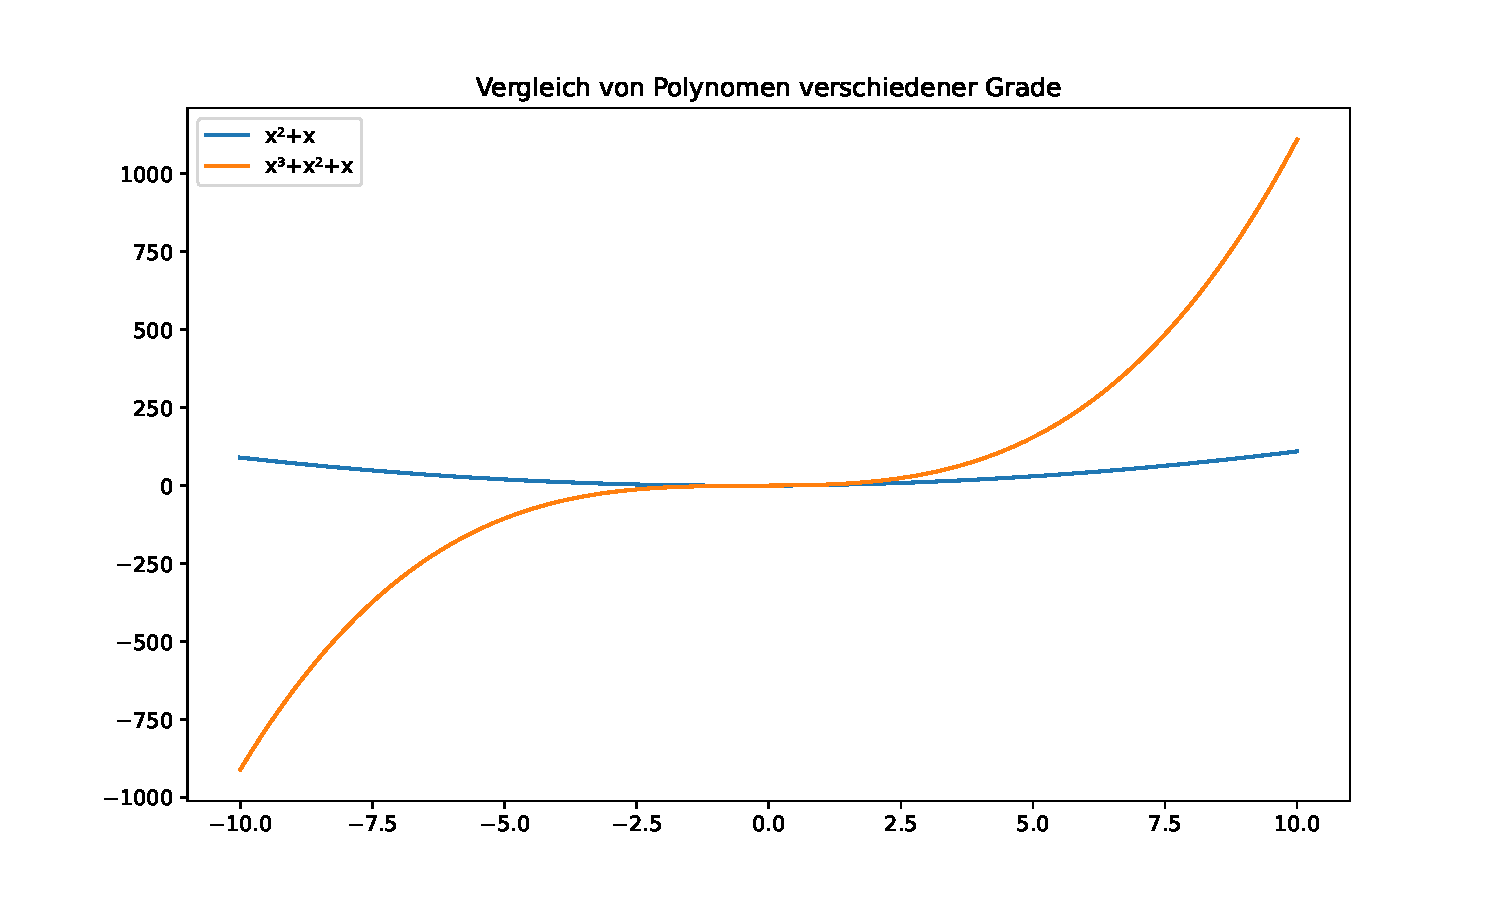
\includegraphics[width=0.7\textwidth]{Graphics/ComparissonDifferentPolDegrees.pdf}
  \caption{Vergleich von Polynomen verschiedener Grade}
  \label{fig:PolynomeVerschiedeneGrade}
\end{figure}

Um ein Verständnis für die Verluste zu bekommen, ist in \autoref{fig:RekonstruktionPoly} ein Beispiel einer rekonstruierten Zeitreihe zu finden, die mit einer Segmentlänge von 100 stückweise polynomiell komprimiert wurde.
\begin{figure}[bth] 
  \centering
  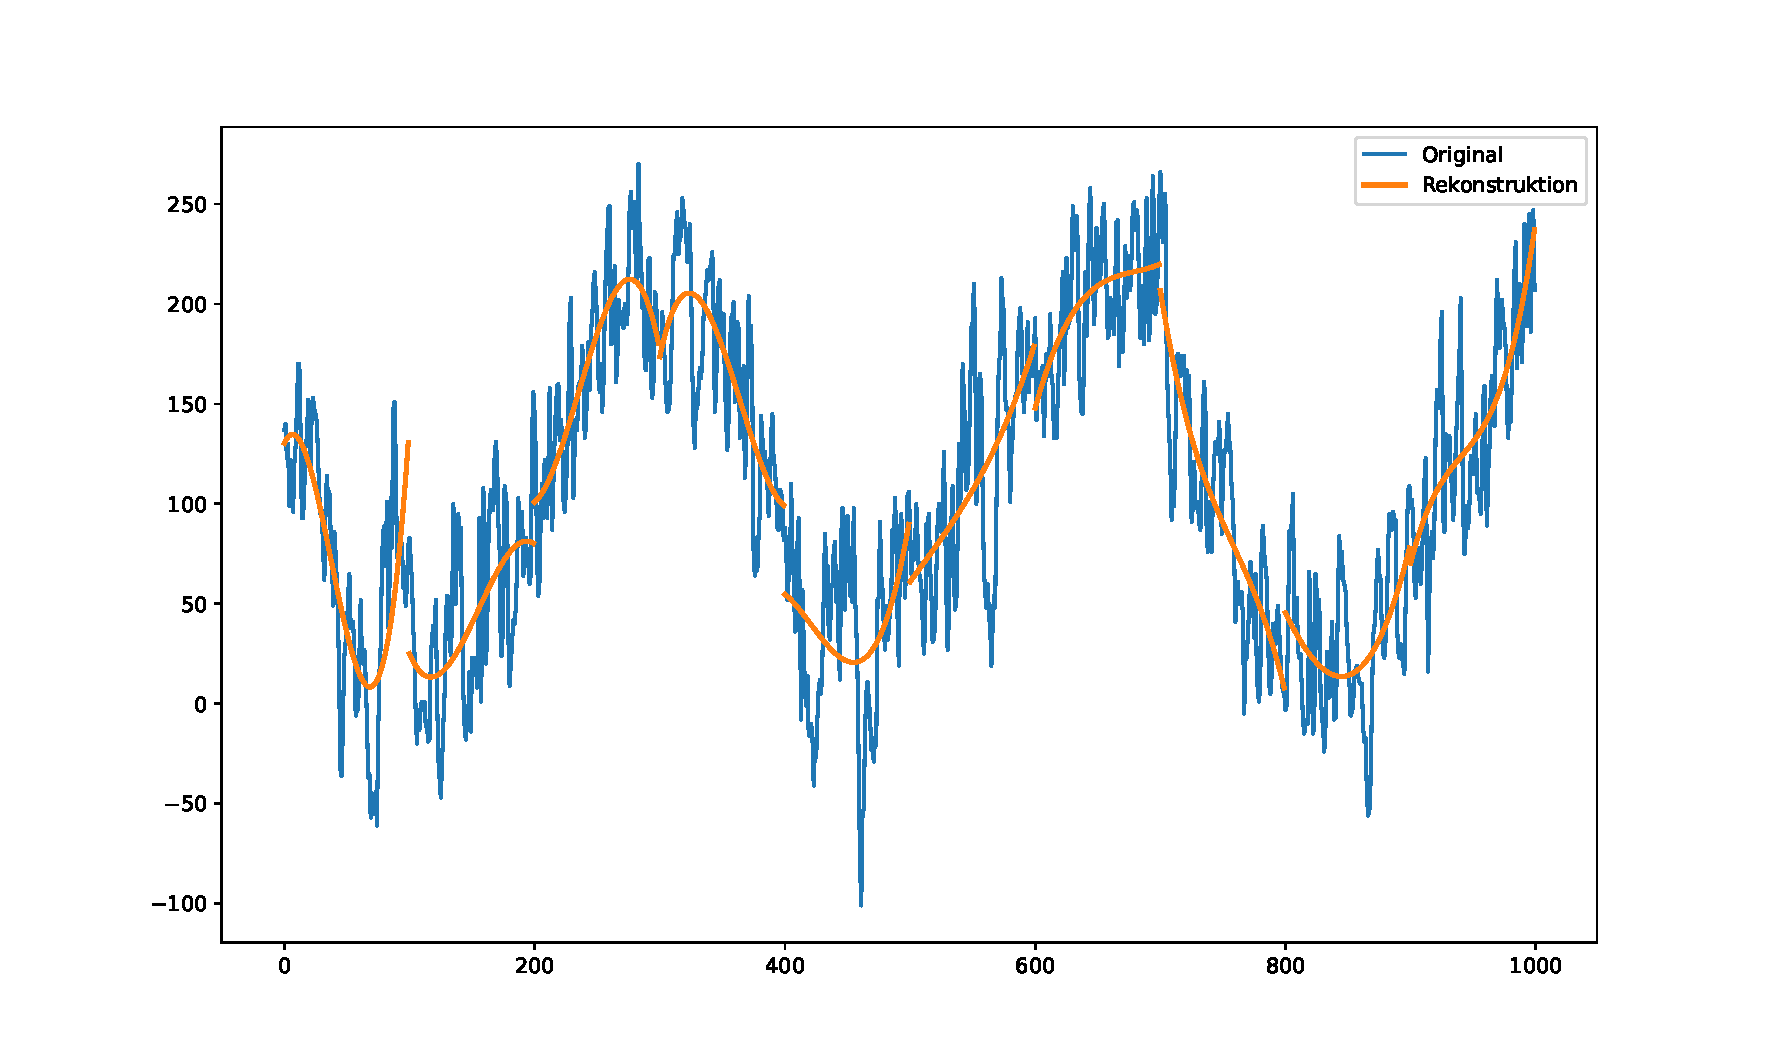
\includegraphics[width=0.7\textwidth]{Graphics/RekonstruktionPoly.pdf}
  \caption{Rekonstruktion einer mit Grad 3 stückweise polynomiell komprimierten Zeitreihe}
  \label{fig:RekonstruktionPoly}
\end{figure}

\subsection{Stückweise lineare Approximation}
Die stückweise lineare Approximation stellt einen Spezialfall der stückweisen polynomiellen Approximation dar, bei dem ausschließlich Polynome ersten Grades (also lineare Funktionen) zur Approximation der Segmente verwendet werden.
Durch die Beschränkung auf Grad 1 ergibt sich eine einfachere Funktionsform sowie geringerer Rechenaufwand, jedoch unter Umständen auch eine schlechtere Approximation komplexer Verläufe im Vergleich zu höhergradigen polynomiellen Approximationen.

Um ein Verständnis für die Verluste zu bekommen, ist in \autoref{fig:RekonstruktionLinear} ein Beispiel einer rekonstruierten Zeitreihe zu finden, die mit einer Segmentlänge von 100 stückweise linear komprimiert wurde.
\begin{figure}[bth] 
  \centering
  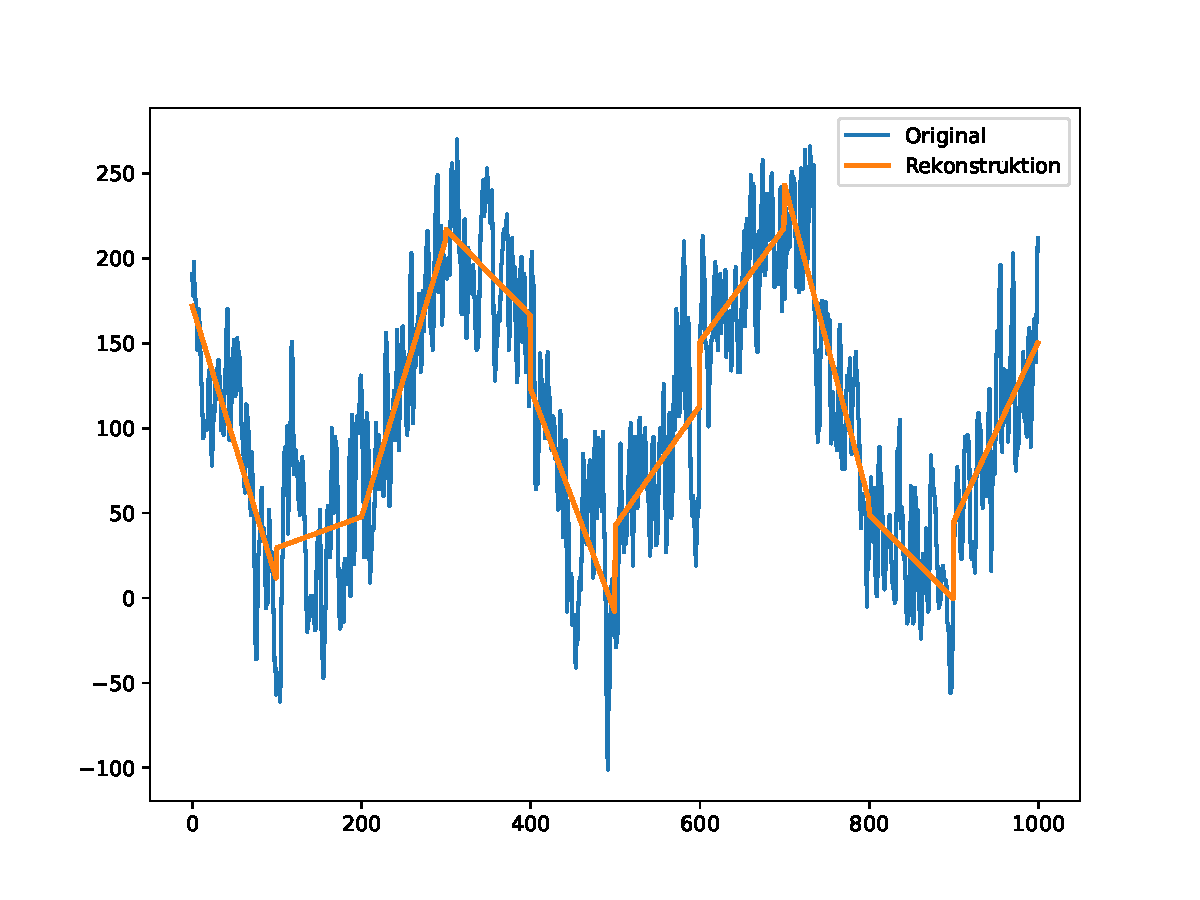
\includegraphics[width=0.7\textwidth]{Graphics/RekonstruktionLinear.pdf}
  \caption{Rekonstruktion einer stückweise linear komprimierten Zeitreihe}
  \label{fig:RekonstruktionLinear}
\end{figure}

\subsection{Diskrete Fourier-Transformation}\label{subsec:dft}
Die \ac{DFT} ist ein mathematisches Verfahren zur Zerlegung einer endlichen, diskreten Zeitreihe in ihre Frequenzteile. Das heißt, für eine gegebene Zeitreihe $[(t_0,x_0),(t_1,x_1),\ldots,(t_{n-1},x_{n-1})]$ gibt \acs{DFT} eine neue Liste mit den Frequenzen von 0 bis $n-1$ zurück. Für diese Transformation ist folgende Formel definiert:
\[y_k=\sum_{\ell=0}^{n-1}x_\ell\,e^{i\,\tfrac{2\pi k}{n}\,\ell},\]
wobei $[y_0,y_1,\ldots,y_{n-1}]$ die neue Liste ist und $i$ die imaginäre Einheit.

Was dieses Verfahren tut, lässt sich gut an einem Beispiel zeigen. In \autoref{fig:dftKomplettBeispiel} sieht man in Grün ein Signal, das aus drei sich überlagernden Frequenzen erstellt wurde. Die blauen Punkte sind zwölf Messpunkte einer Zeitreihe, die dieses Signal abgetastet hat, und die orangenen Kreuze sind die Beträge des Ergebnisses der \acs{DFT}. 
\begin{figure}[bth] 
  \centering
  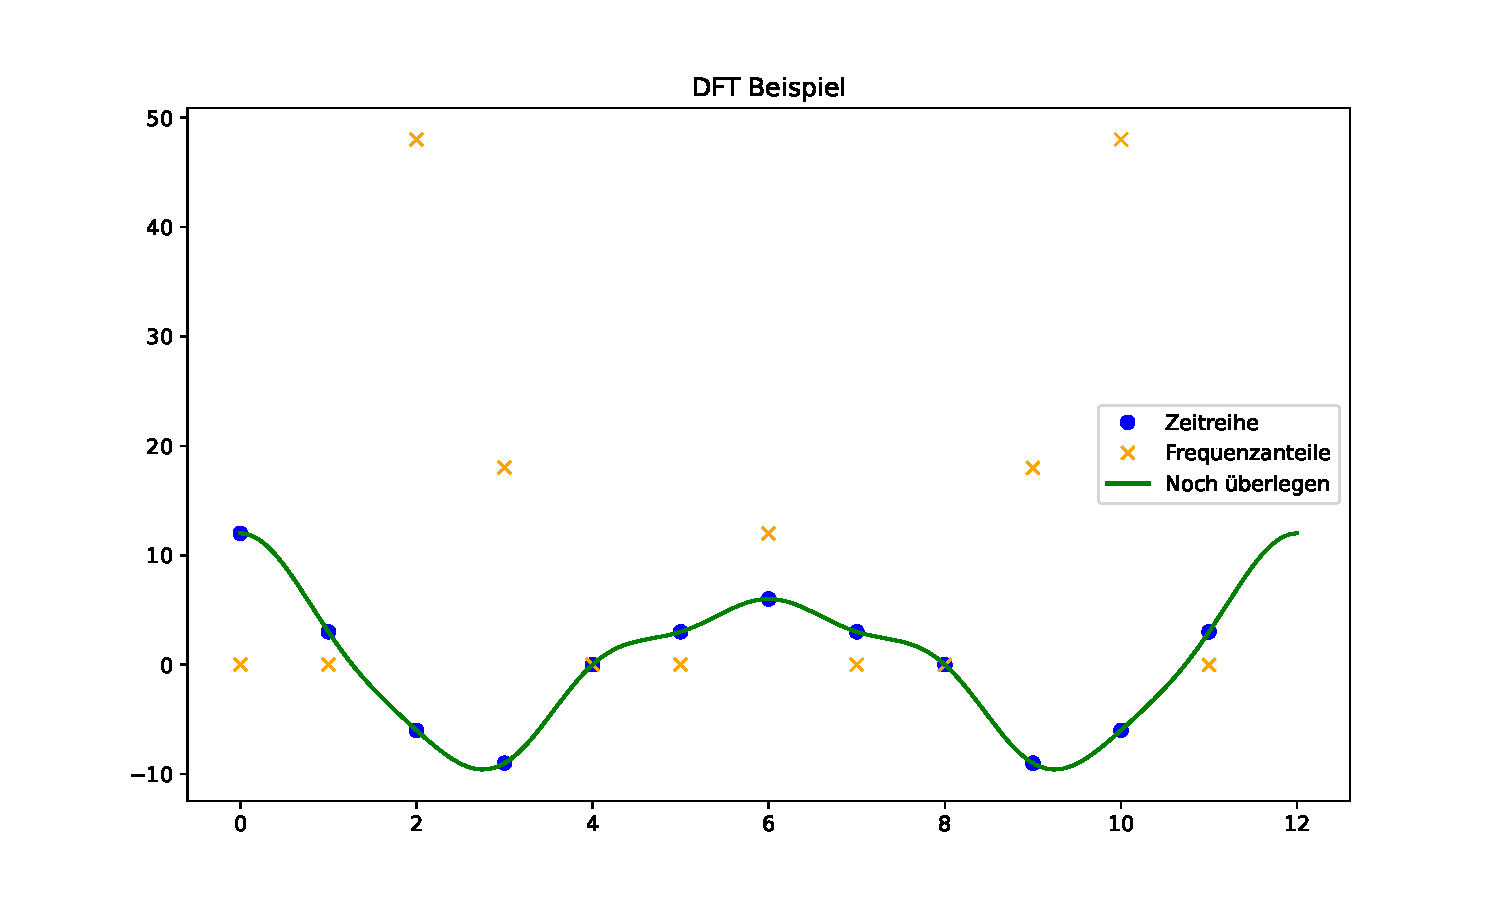
\includegraphics[width=0.7\textwidth]{Graphics/DFTExample1.pdf}
  \caption{Beispiel einer diskreten Fourier"=Transformation}
  \label{fig:dftKomplettBeispiel}
\end{figure}

In \autoref{fig:dftEinzelneFrequenzen} sieht man nun die drei ursprünglichen Frequenzen, die überlagert das Signal aus \autoref{fig:dftKomplettBeispiel} ergeben. Die blauen Punkte und orangenen Kreuze zeigen auch hier das abgetastete Signal beziehungsweise die Beträge des Ergebnisses der \acs{DFT}. Durch die Aufteilung in die drei einzelnen Bilder wird klar, was die \acs{DFT} eigentlich macht. Sie extrahiert aus dem ursprünglichen Signal diese drei Frequenzen und speichert mittels einer komplexen Zahl Informationen über die Amplitude und Phasenverschiebung der jeweiligen Frequenz. So sieht man in \autoref{subfig:dft2}, dass beide Amplituden bei 48 liegen. Da die \acs{DFT} diese Werte nicht normalisiert, müssen sie, nachdem sie addiert wurden, durch $n=12$ dividiert werden. Wir erhalten eine Amplitude von 8, was durch Betrachtung des grünen Graphens bestätigt werden kann. Selbiges gilt für \autoref{subfig:df3} und \autoref{subfig:dft4}, wo die addierten Amplituden 36 beziehungsweise 12 ergeben und die normierten 3 beziehungsweise 1.
\begin{figure}[bth]
  \subfloat[Erste Frequenz]{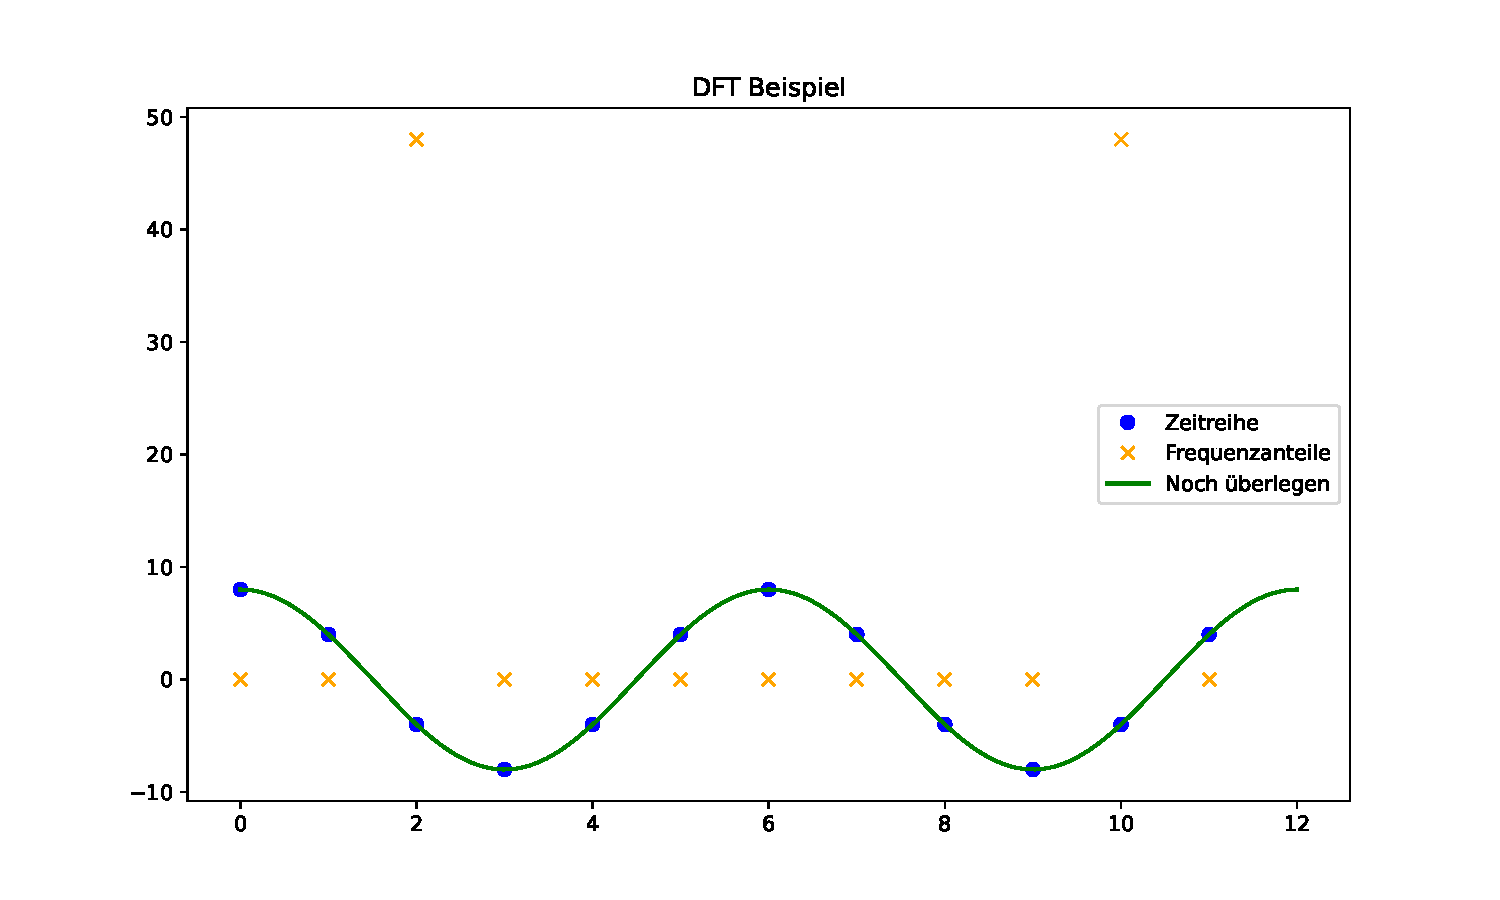
\includegraphics[width=0.49\textwidth]{Graphics/DFTExample4.pdf}\label{subfig:dft2}}\hfill
  \subfloat[Zweite Frequenz]{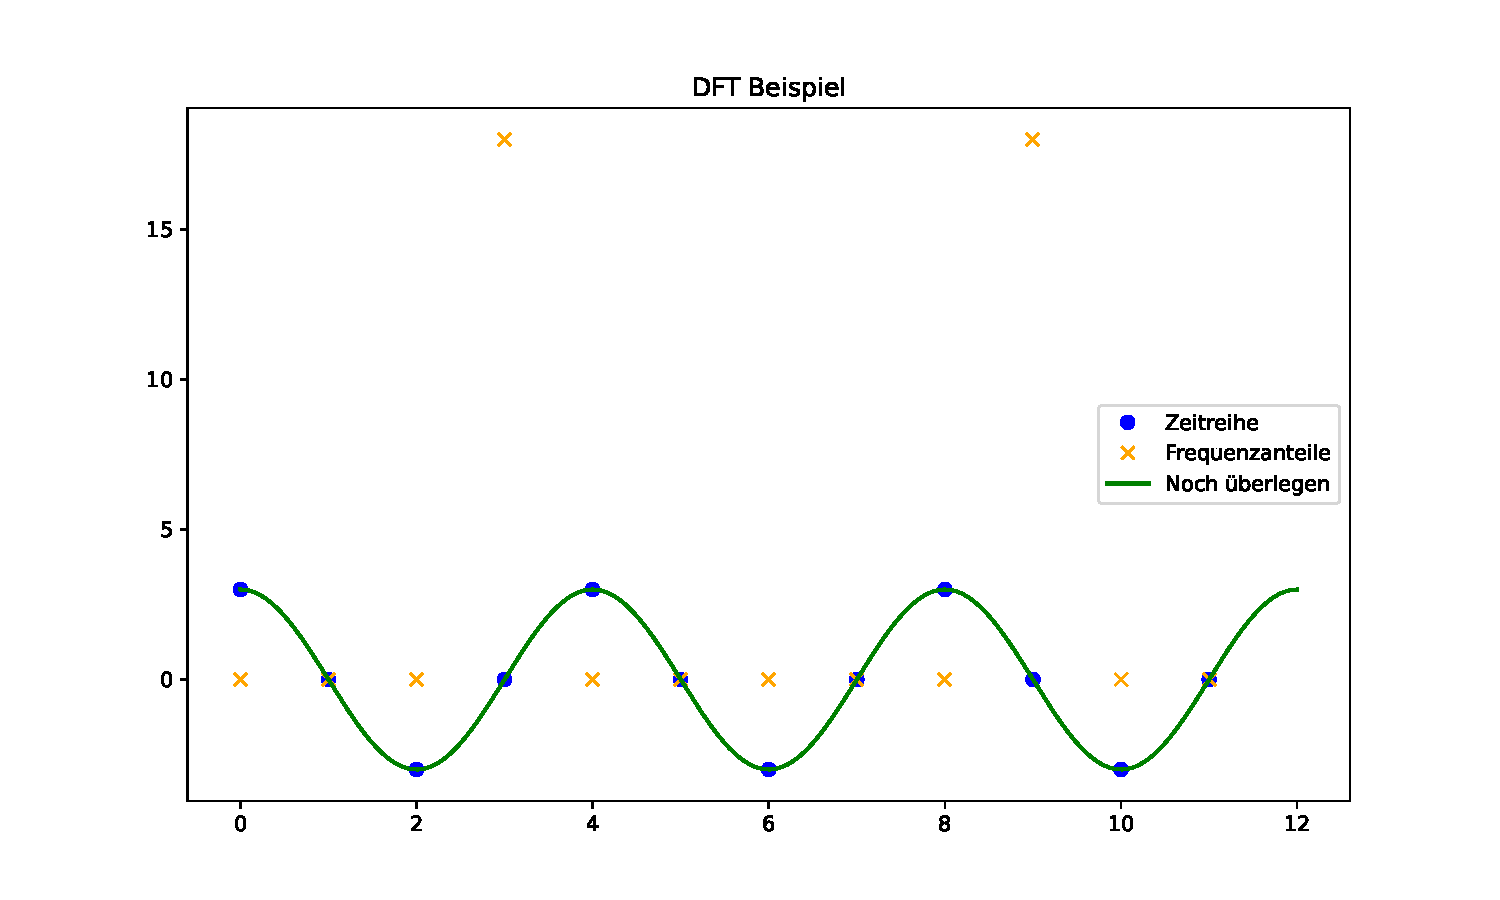
\includegraphics[width=0.49\textwidth]{Graphics/DFTExample3.pdf}\label{subfig:df3}}\hfill
  \centering\subfloat[Dritte Frequenz]{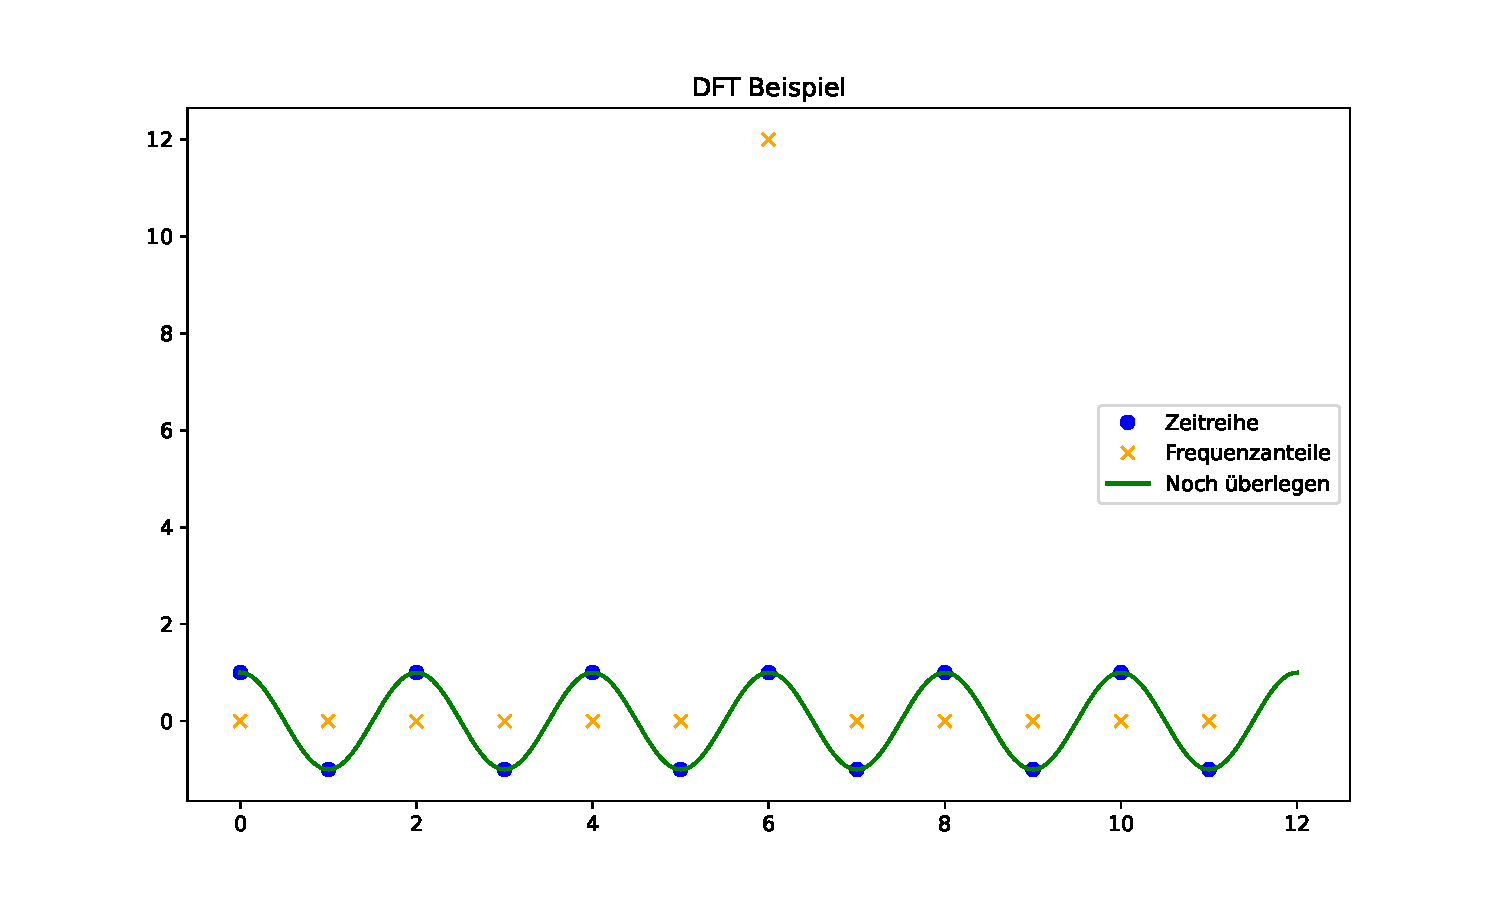
\includegraphics[width=0.49\textwidth]{Graphics/DFTExample2.pdf}\label{subfig:dft4}}
  \caption{Ursprüngliche Frequenzen der Überlagerung aus \autoref{fig:dftKomplettBeispiel}}
  \label{fig:dftEinzelneFrequenzen}
\end{figure}

Zum besseren Verständnis der am Anfang genannten Formel wird in diesem Abschnitt nun näher auf die Mathematik dahinter eingegangen. In der Formel handelt es sich wegen der imaginären Einheit $i$ um komplexe Zahlen. Diese bestehen aus einem Realteil $a$ und einem Imaginärteil $b$, also in der Form $a + ib$. Sie können allerdings auch als Punkt in einer zweidimensionalen Ebene interpretiert werden, dann liegt der Realteil typischerweise auf der x-Achse und der Imaginärteil auf der y-Achse. Außerdem gibt es die Exponentialform $a+ib=re^{i\varphi}$, wobei $r$ der Abstand vom Ursprung zum Punkt $(a,b)$ ist und $\varphi$ der Winkel, den diese Strecke mit der positiven x-Achse einschließt. $r$ wird auch Betrag genannt und wird folgendermaßen berechnet: $r=\sqrt{a^2+b^2}$. Setzt man nun $r=1$ und lässt $\varphi$ von 0 bis $2\pi$ laufen, erhält man einen Einheitskreis. Unterteilt man diesen Kreis jetzt in $n$ gleich große Abschnitte, so kann man mit $e^{i\frac{2\pi k}{n}}$ über $n$ diskrete Punkte iterieren, wobei $k$ eine natürliche Zahl von 0 bis $n-1$ ist. Auffallen dürfte an dieser Stelle, dass dieser Term dem aus der obigen Summenformel entspricht. Setzt man also nun $n=12$, entsprechend unseres Beispiels in \autoref{fig:dftKomplettBeispiel}, so erhält man einen Einheitskreis, der mit dem in \autoref{fig:komplexerEinheitskreis} übereinstimmt. Diese 12 Punkte werden dann mit den restlichen Termen der \acs{DFT}, nämlich den Datenpunkten gewichtet. Diese Darstellung als komplexe $e$"=Funktion entspringt der Idee eine Funktion als Linearkombination von Cosinus"= und Sinus"=Termen anzunähern. Das legt also folgenden Ansatz nah: \[f(x)\sim\frac{a_0}{2}+\sum_{\ell=1}^{\infty}\Bigl(a_\ell\cos(\ell x)+b_\ell\sin(\ell x)\Bigr).\] Da $\cos x = (e^{ix}+e^{-ix})/2 \text{ und } \sin x = (e^{ix}-e^{-ix})/2i$, lässt sich dieser Ansatz dann in die komplexe Fourierreihe überführen, die allgemein als \[f(x) \sim \sum_{\ell = -\infty}^\infty c_\ell e^{i\ell x}\] geschrieben werden kann und diskretisiert die Formel der \acs{DFT} ergibt, die deutlich kompakter und einfacher zu berechnen ist als mit den trigonometrischen Funktionen. Auf die Herleitung zwischen dem ersten Ansatz und der \acs{DFT} möchten wir an dieser Stelle nicht eingehen und verweisen hierfür auf das Lehrmaterial von Stefan Krause \cite{fourierundwavelet}.

Für die Abschätzung der Laufzeit ergibt sich, dass für jedes Element der Zeitreihe, also $n$"=mal, die Summenformel von 0 bis $n-1$ berechnet werden muss, und somit die Laufzeit in $O(n^2)$ liegt, was zu langsam für große Zeitreihen ist. Die Fast Fourier"=Transformation löst dieses Problem, indem es einen Algorithmus implementiert, der die Werte der \acs{DFT} effizienter berechnet. Die Laufzeit liegt dann nur noch in $O(n\log n)$, übertragen auf Sortieralgorithmen wäre das ein Wechsel von Bubblesort zu MergeSort. Auf die Implementierung der Fast Fourier"=Transformation wird in dieser Arbeit nicht weiter eingegangen, da es lediglich eine Optimierung der \acs{DFT} ist und diese nicht relevant zum Verständnis des Inhalts ist.
\begin{figure}[bth] 
  \centering
  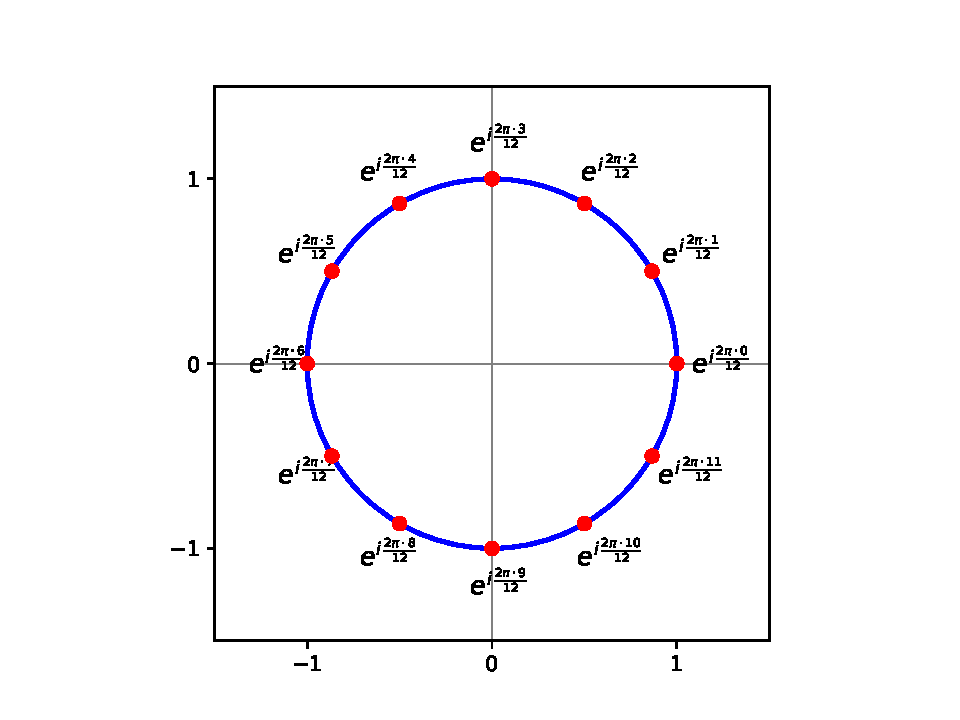
\includegraphics[width=0.7\textwidth]{Graphics/KomplexerEinheitskreis.pdf}
  \caption{Einheitskreis mit zwölf gleich großen Abschnitten}
  \label{fig:komplexerEinheitskreis}
\end{figure}

Um ein Verständnis für die Verluste zu bekommen, ist in \autoref{fig:RekonstruktionFourier} ein Beispiel einer rekonstruierten Zeitreihe zu finden, die mit der Fast"=Fourier Transformation komprimiert wurde, indem nur die 10\% der Frequenz gespeichert wurden, die den größten Betrag zum Signal beitragen.
\begin{figure}[bth] 
  \centering
  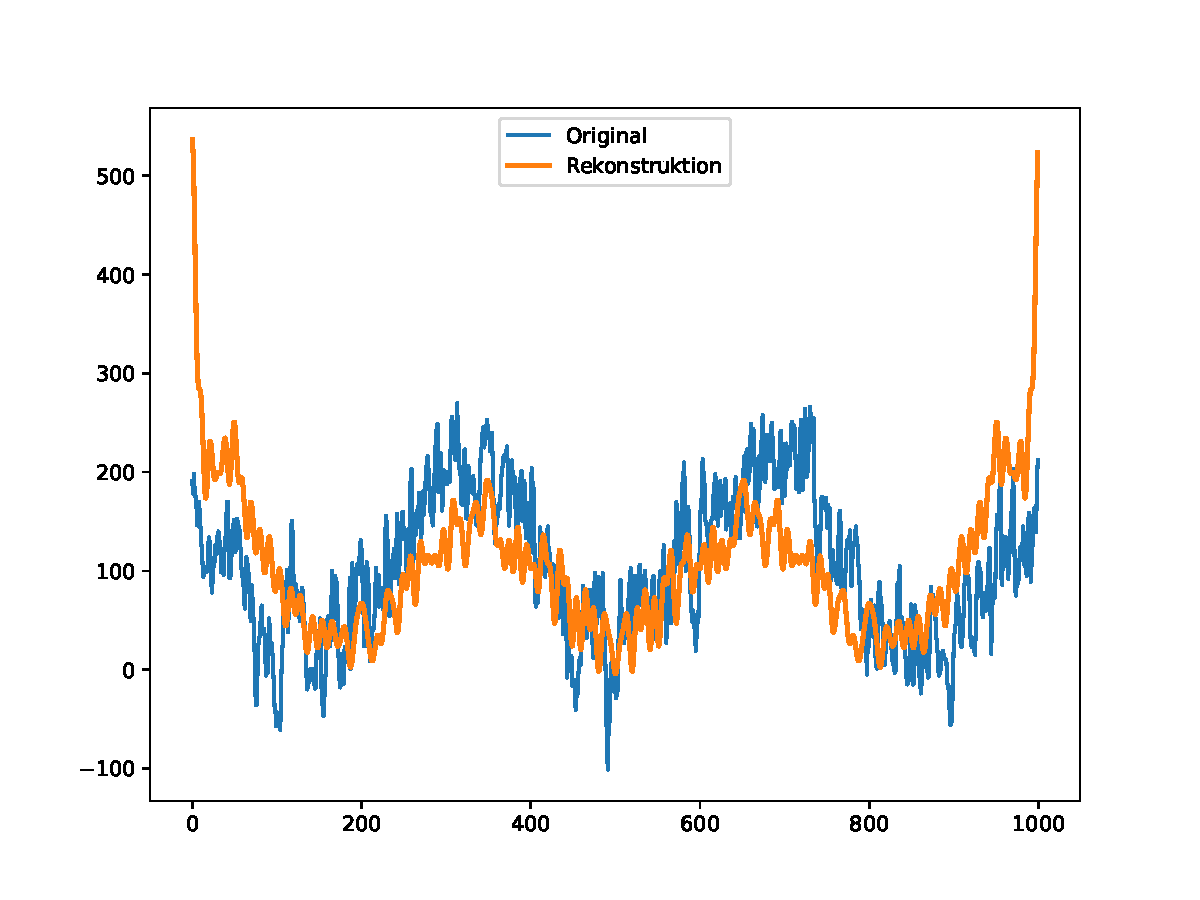
\includegraphics[width=0.7\textwidth]{Graphics/RekonstruktionFourier.pdf}
  \caption{Rekonstruktion einer mit der Fast"=Fourier"=Transformation komprimierten Zeitreihe}
  \label{fig:RekonstruktionFourier}
\end{figure}

\subsection{Diskrete Wavelet"=Transformation}
Im vorherigen Abschnitt haben wir gesehen, dass die \acs{DFT} ein Signal, beziehungsweise in unserem Fall eine Zeitreihe, als Linearkombination von Cosinus"= und Sinus"=Funktionen mit verschiedenen Vielfachen der Grundfrequenz beschreibt. Diese sogenannten Basisfunktionen besitzen eine sogenannte Frequenzlokalität, das bedeutet an den Koeffizienten $a_\ell$ und $b_\ell$ beziehungsweise $c_\ell$ kann man ablesen wie stark ein Vielfaches der Grundfrequenz vorhanden ist. Allerdings gilt diese Information global für das gesamte Signal, was bedeutet es gibt keine sogenannte zeitliche Lokalität, die Informationen darüber enthält, wo diese Schwingungen auftreten.

Dieses Problem versucht die Wavelet"=Transformation zu beheben, indem es ein Signal in lokalisierte Basisfunktionen zerlegt (Wavelets), die sowohl verschiedene Frequenzen, als auch verschiedene Lokalitäten abbilden können. Von diesen Basisfunktionen gibt es verschiedene Typen, so nutzen wir in der Implementierung Daubechies"=Wavelets, weil sie die mit am meisten genutzten sind und auch in den Beispielen der verwendeten Bibliothek vorkommen. Um allerdings das Prinzip zu veranschaulichen, nutzen wir die Haar"=Wavelets, da sie einfacher zu verstehen und zu veranschaulichen sind.

Aus dem in \autoref{subsec:dft} bereits erwähnten Skript und von Joran Berg et al.\cite{wavelets} entnehmen wir folgendes: Die Haar"=Wavelet"=Basis lautet allgemein: \[ \{\phi\} \cup \bigcup_{k=1}^\ell \Bigl\{ 2^{(k-1)/2} \, \psi \bigl( 2^{k-1} x - j \bigr) \Bigm| 0 \leq j < 2^{k-1} \Bigr\} \,, \]
wobei $\ell=\lfloor \log_2(n) \rfloor$. $\phi$ ist hierbei das erste Element und ganz links in \autoref{fig:vierbasiselemente} zu sehen. $\psi$ ist das zweite Element und in der Abbildung an zweiter Stelle von links zu sehen. Die anderen Elemente entstehen also aus diesem Element heraus, indem mit $2^{k-1}x-j$ die Funktion auf der x"=Achse verschoben und in x"=Richtung skaliert wird und indem mit $2^{(k-1)/2}$ die Funktion normiert wird. Die beiden rechten Funktionen in der Abbildungen entstehen also, indem $\psi$ auf die Hälfte gestaucht wird und ein mal unverändert, ein mal um $0,5$ nach rechts verschoben wird. Die kontinuierliche Wavelet"=Transformation lautet dann: \[f(x) \sim a_0 \, \phi(x) + \sum_{k=1}^\infty \sum_{j=0}^{2^{k-1}-1} a_{k,j} \, \psi_{k,j}(x) \,.\] Die erste Summe läuft mit $k$ über die Frequenzkomponenten, ähnlich wie bei der Fourierreihe, während die zweite Summe mit $j$ zu jeder Frequenz durch die verschobenen Basisfunktionen die zeitliche Lokalität herstellt und die jeweilige Basisfunktion mit dem Koeffizienten $a_{k,j}$ gewichtet.
\begin{figure}[h]
  \waveletfunction{(0, 1) -| (1, 0)}%
  \hfill%
  \waveletfunction{(0, 1) -| (0.5, -1) -| (1, 0)}%
  \hfill%
  \waveletfunction{(0, 1.414) -| (0.25, -1.414) -| (0.5, 0)}%
  \hfill%
  \waveletfunction{(0.5, 1.414) -| (0.75, -1.414) -| (1, 0)}%
  \caption{Erste vier Basiselemente der Haar"=Wavelets}
\end{figure}\label{fig:vierbasiselemente}
\renewcommand{\waveletfunction}[1]{%
 \begin{tikzpicture}[x = 20mm, y = 20mm]
  %\draw (-0.45, -1.5) rectangle (1.2, 1.7);
  \useasboundingbox (-0.45, -1.5) rectangle (1.2, 1.7);
  \draw [->] (-0.1, 0) -- (1.2, 0);
  \draw [->] (0, -1.5) -- (0, 1.7);
  \tikztextr{1.2}{0.15}{$x$}
  \tikztextl{0.075}{1.65}{$y$}
  \tikztextc{0}{-0.15}{$0$}
  \tikztextc{0.5}{-0.15}{$0{,}5\ell$}
  \tikztextc{1}{-0.15}{$\ell$}
  \tikztextr{-0.075}{-1}{$-c$}
  \tikztextr{-0.075}{1}{$c$}
  \draw [blue, thick] (-0.05, 0) -| #1 -- (1.05, 0);
 \end{tikzpicture}%Erste vier Basiselemente der Haar"=Wavelets in PyWavelets
}

In der von uns verwendeten Bibliothek PyWavelets \cite{pyWavelets} werden allerdings nicht wie in der kontinuierlichen Wavelet"=Transformation die Koeffizienten jeder verschobenen Basisfunktion berechnet, sondern durch die Diskrete Wavelet"=Transformation die sogenannten Approximations"=Koeffizienten und die Differenz"=Koeffizienten. Die Approximations"=Koeffizienten $cA$ entsprechen beim Haar"=Wavelet $cA_k = 1/\sqrt{2}(x_{2k} + x_{2k+1})$, also eine Mittlung des Originalsignals. Die Differenz"=Koeffizienten $cD$ entsprechen beim Haar"=Wavelet $cD_k = 1/\sqrt{2}(x_{2k}-x_{2k+1})$, also wie stark die Werte von der Mittelung abweichen. Dadurch dass immer zwei Werte miteinander kombiniert werden, entspricht die Anzahl von $cA$ und $cD$ jeweils der Hälfte der Anzahl der ursprünglichen diskreten Werte. Zum Komprimieren von Signalen nutzen wir die $cA$ und führen so viele Iterationen der Wavelet"=Transformation auf ihnen durch, bis der gewünschte Kompressionsgrad erreicht ist. Die $cD$ werden in unserem Fall ignoriert.
%\begin{figure}[h]
%  \waveletfunction{(0, 1) -| (1, 0)}%
%  \hfill%
%  \waveletfunction{(0, 1) -| (0.25, -1) -| (0.5, 0)}%
%  \hfill%
%  \waveletfunction{(0.5, 1) -| (0.75, -1) -| (1, 0)}%
%  \caption{Skalierungs"= und Wavelet"=Funktionen in PyWavelets}
%\end{figure}\label{fig:basispywavelets}

Um ein Verständnis für die Verluste zu bekommen, ist in \autoref{fig:RekonstruktionWavelet} ein Beispiel einer rekonstruierten Zeitreihe zu finden, die mit vier Iterationen der diskreten Wavelet"=Transformation komprimiert wurde.
\begin{figure}[bth] 
  \centering
  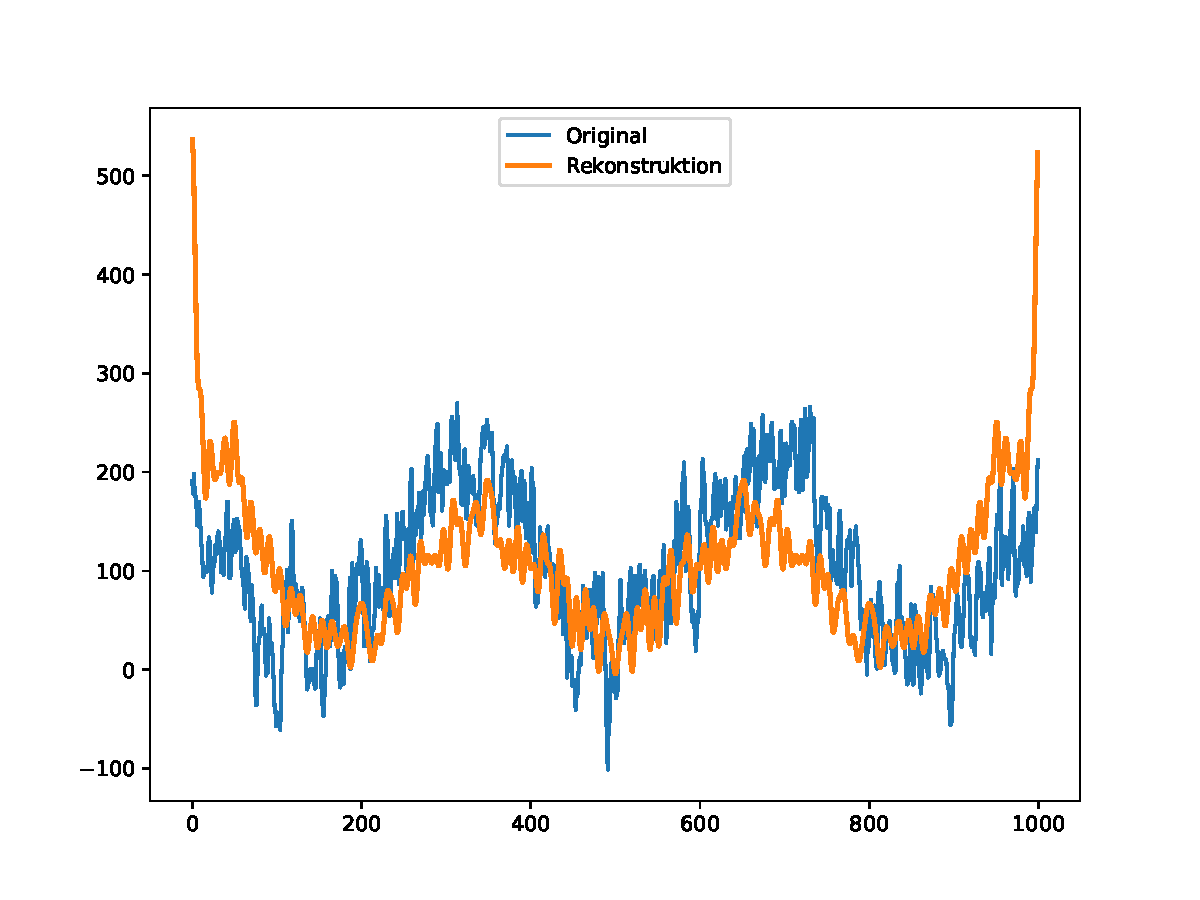
\includegraphics[width=0.7\textwidth]{Graphics/RekonstruktionFourier.pdf}
  \caption{Rekonstruktion einer mit der diskreten Wavelet"=Transformation komprimierten Zeitreihe}
  \label{fig:RekonstruktionWavelet}
\end{figure}